
Science is understanding the world -- $\theta \epsilon \omega \rho \iota \alpha $; art is affecting the world -- $ \pi \rho \alpha \xi \iota \sigma $.
Outreach for scientists is a matter not just of connecting with colleagues in the academy, as C.P. Snow~\cite{SnowTwoCultures} said, bridging the Two Cultures.
It is reaching back to our innate humanity and the world from which it came, the universe trying to understand itself. 
No single exhibit reaches this goal, though we do our best with rubber sheets, lasers, and interactive light and sound sculptures. 
Diligence nonetheless can spark curiosity.
LIGO has made concerted efforts to reach further into the universe with ever more sensitive technology, and in leadup to the World Science Festival (WSF) exhibit on LIGO in 2010 in Manhattan, we tenaciously developed more sophisticated exhibits to connect with a broader audience. 

Many kinds of exhibits have been made to showcase aspects of general relativity.
Rubber sheets of `spacetime' are familiar to many museum-goers; the WSF had one too, with a central mass to deform the sheet like gravity and a smaller marble that could `orbit' it.
More central to the WSF exhibit about LIGO, however, was an interferometer.
Requiring a strong laser, stable alignment, and asymmetric-length arms to great a distinct bullseye fringe pattern, this interferometer's design, installation and commissioning was the responsibility of the author.
As a microcosm of the challenges mentioned in the introduction, the WSF offers humbling insight into both gravitational wave astronomy and its significance to the public.


    \section{Prototypes: travelling kiosks and the Ann Arbor Hands-On Museum} 
    \label{prototypes}

        %Prototypes: Ann Arbor Hands-On Museum and travelling kiosk.

The Michigan Gravitational Wave Group (MGWG) came to the WSF project with experience.
Ramon Armen had developed a small interferometer with Goetz and Riles, approximately 50 cm square, that integrated into a kiosk design.
This kiosk was developed in collaboration with the Ann Arbor Hands-On Museum exhibits director John Bowditch.
Charlie Stout wrote an interactive Flash program for the kiosk.

In the small interferometer, a 0.9 mW Helium-Neon laser beam passes through a beam spliter, travels down two arms of slightly different length, and reflects off retroreflecting mirrors at the end of each arm.
The retroreflectors contain three mutually-perpendicular planes that redirect the beam parallel and opposite to its incident path, offset by twice the distance from the retroreflector corner.
Retroreflectors are more robust against misalignment than flat mirrors, although reflected images cast a six-spoke shadow pattern due to the three intersecting lines between the planes.
Slight beam offset away from the center avoids these spokes.
These optical elements are mounted on a portable breadboard with pre-fabricated optical table-style holes.
Recombined at the beam splitter, some light goes to a beam dump while the remainder is directed to a screen.
As the path length of the beams and consequent phase delay changes -- due to thermal expansion of the breadboard, vibrations, and so on -- the screen shows a fluctuating fringe pattern that illustrates the constructive and destructive interference of light waves.
Mismatched wavefront curvatures, arising from travel along the different-length arms, give this fringe pattern a well-defined circular shape.
Speakers, when used, let exhibit-goers hear how vibrations, which they themselves can make by tapping on the kiosk, reverberate through the mirrors and and be both seen on-screen and heard as fringes pass the photodiode. 
In the kiosk, a swinging lever arm, controlled by whoever stands at the kiosk, can block the light from one of the arms, blocking the inteference; the user can see that the fringe pattern indeed comes from the wave nature of light.

A full set of parts for the kiosk interferometer was assembled by the author (Table~\ref{WSF_IFO_BOM}) according to Figure~\ref{kiosk_ifo_schematic} in the process of building another unit.
This additional interferometer went on travelling exhibition, organized by Marco Cavaglia of the University of Mississipi, across the United States starting with the 2009 WSF, and it was most recently on display at Stanford University in August 2014.
It is durable, but for the LIGO `Astronomy's New Messengers' 2010 WSF exhibit, the MGWG crafted something more dramatic.

    \subsubsection{Bill of materials: interferometer parts}

Equipment as below builds one interferometer for our Ann Arbor Hands-On
Museum outreach design. 
We include company names, part numbers, quantities, and
prices, after the work done in 2008 by Ramon Armen. 
Assembly follows from the
work detailed on

\url{http://gallatin.physics.lsa.umich.edu/~keithr/outreach/}, 

in particular the parts list (plain text file) written by the author,

\url{http://gallatin.physics.lsa.umich.edu/~gmeadors/Interferometer_parts},

and the schematic 

\url{http://gallatin.physics.lsa.umich.edu/~keithr/outreach/ifo_schematic.jpg}. 

See Table~\ref{WSF_IFO_BOM} for details on parts from each of the manufacturers: \\
CVI Melles-Griot\footnote{CVI Melles-Griot: \href{tel:15052969541}{\texttt{+1 505 296 9541}}; press 2 at menu},\\
Edmund Optics\footnote{Edmund Optics: \href{tel:18003631992}{\texttt{+1 800 363 1992}}; press 1 (?) for sales},\\
OptoSigma\footnote{OptoSigma: \href{tel:19498515881}{\texttt{+1 949 851 5881}} }, and\\
ThorLabs\footnote{ThorLabs: \href{tel:19735797227}{\texttt{+1 973 579 7227}}; press 1 (?) for sales}.

\begin{table}
\begin{center}
%CVI Melles-Griot: 1 505 296 9541; press 2 at menu \\
\begin{tabular}{l l l l}
\hline
Description     & Part Number$^1$     & Quantity   & Approximate Unit Price\\
\hline
HeNe laser      & 05 LLR 811-249  & 1         & \$320 \\
Laser stand     & 07 LHE 001      & 1         & \$40 \\
%\end{tabular}
%Edmund Optics: 1 800 363 1992; press 1 (?) for sales \\
%\begin{tabular}{l l l l}
\hline
Description     & Part Number$^2$     & Quantity &  Approximate Unit Price\\
\hline
-50 lens        & NT32-996        & 1        &  \$27 \\
-25 lens        & NT32-992        & 1        &  \$27 \\
Lens holder     & NT54-980        & 2        &  \$33.00\\
%\end{tabular}
%OptoSigma: 1 949 851 5881 
%\begin{tabular}{l l l l}
\hline
Description  &   Part Number$^3$  &   Quantity  & Approximate Unit Price\\
\hline
Beam splitter  &  038-0590     &   1    &      \$250\\
Retroreflector & 055-2340      &  2     &     \$289.00\\
"" holder      &  113-0045     &   2    &      \$69.00\\
%\end{tabular}
%\begin{tabular}{l l l l}
\hline 
Description   &  Part Number$^4$  &   Quantity   & Approximate Unit Price\\
\hline
BS holder    &   LMR2         &   1       &   \$23.50\\
Rotary mount &   RP01         &   1       &   \$91.00 \\
1.0" holder  &   PH1-ST       &   1       &   \$7.03\\
1.5" holder  &   PH1.5-ST     &   4       &   \$7.22\\
0.75" post   &   TR075        &   1       &   \$4.74 \\
1.0" post    &   TR1          &   4       &   \$4.74 \\
Screw base 1 &   BA1S         &   6       &   \$5.13\\
Screw base 2 &   BA1          &   1       &   \$5.56 \\
%\end{tabular}
%Moreover, the following screws will prove necessary:
%\begin{tabular}{l l l l}
\hline
\hline
Screw type            & Length          & Quantity &\\
\hline
1/4"-20 capped  & 5/4"            & 8\\
1/4"-20 capped  & 3/4"            & 7\\
1/4"-20 set     & 3/8"            & 5\\
\#8-32   set    & 1/2"            & 1\\
\end{tabular}
\caption{Bill of materials (lasers, lenses, mirrors, optic mounts and screws) for interferometer assembly. Manufacturers: $^1$ CVI Melles-Griot, $^2$ Edmund Optics, $^3$ OptoSigma, $^4$ ThorLabs}
\label{WSF_IFO_BOM}
\end{center}
\end{table}

        \begin{figure}
        \begin{center}
        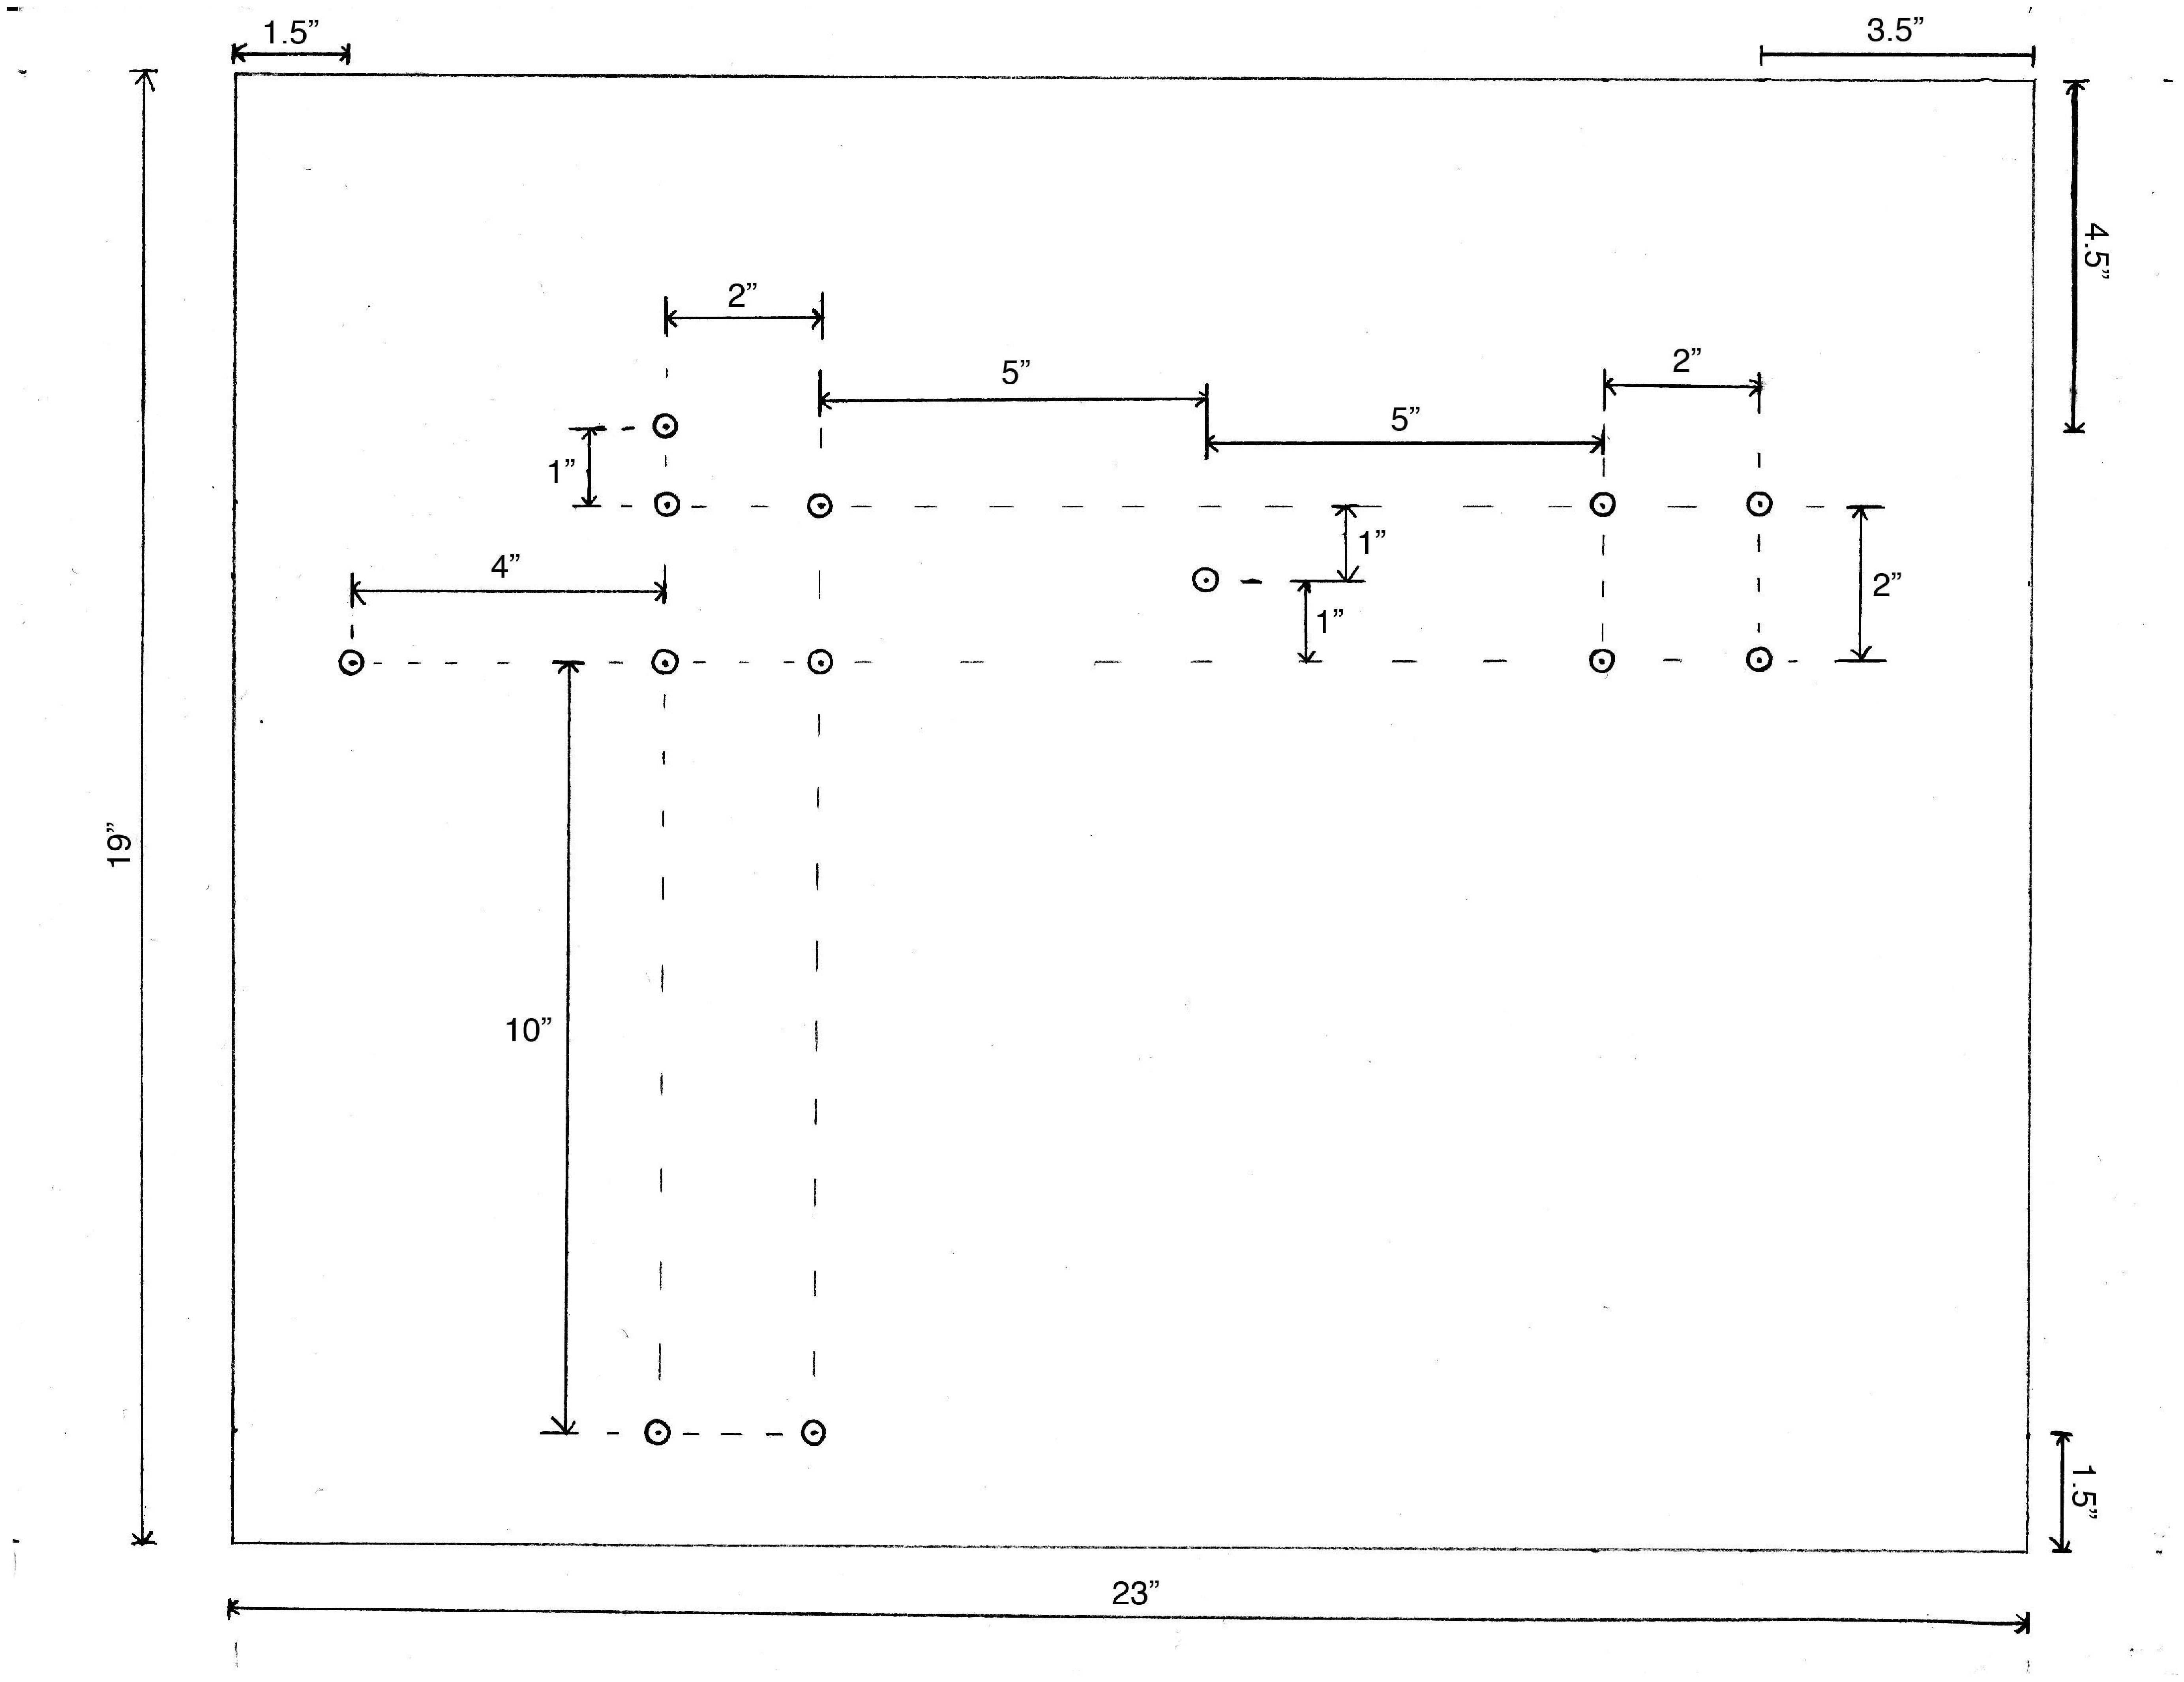
\includegraphics[height=111mm, width=148mm]{ifo_schematic.eps}
        \caption{Kiosk interferometer schematic}
        \label{kiosk_ifo_schematic}
        \end{center}
        \end{figure}

Figure~\ref{kiosk_ifo_schematic} shows the base structural dimensions of this kiosk interferometer.


    \section{World Science Festival interferometer manufacture}
    \label{manufacture}

        %World Science Festival interferometer in isolation.
    
Based on the kiosk interferometer, we collaborated with Cavaglia on a larger interferometer for the WSF.
Displayed first in June 2010 in New York City, the WSF interferometer incorporates new features.
The projection screen was enlarged, made free-standing,
% despite screen manufacture in display section
and incorporates an integrated audio-frequency photodiode connected to a new speaker system.
Laser power is greater to be seen better on the bigger screen, and
laser light has been carefully contained with the use of multiple baffles.
All are contained inside a plexiglass `beam tube' fastened with security screws.
This interferometer stood at the center of the WSF exhibition on LIGO, which received around 2200 visitors in four days.


        \subsection{Laser, optics and display}
        \label{laser_display}

            %Laser and optics (and display).

	\begin{figure}
	\begin{center}
	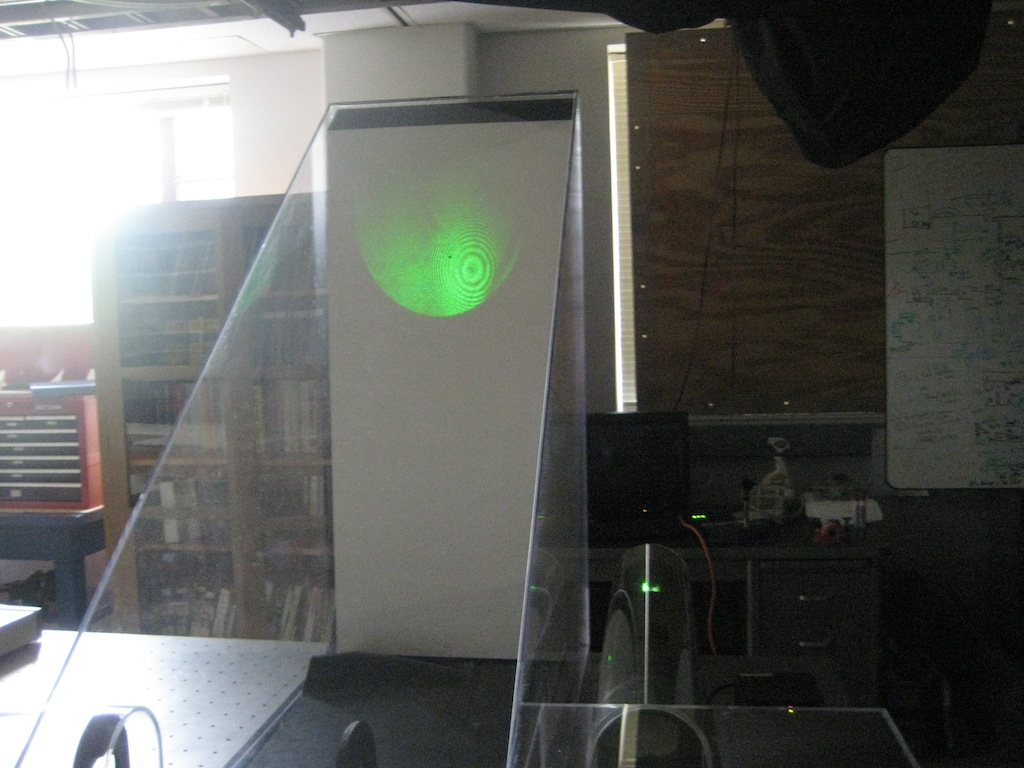
\includegraphics[height=111mm, width=148mm]{WSF_AA_fringes.eps}
	\caption{Interferometer fringes during construction in Ann Arbor}
	\label{WSF_AA_fringes}
	\end{center}
	\end{figure}

Starting from the request for a larger interferometer, the MGWG found a brighter laser with longer coherence length.
Laser Lab Components, Incorporated (LLCI) manufactured a 60 mW Nd-YAG 532 nm laser rated to a coherence length of 50 meters, plenty for the longer path length.
The laser intensity was so bright that we installed a times-8 attenuator to provide just 7.5 mW of visible light.
As the wavelength is green, it is even more visible to the human eye than the red HeNe of the kiosk laser.
To protect visitors' eyes, the author designed a system of eight black-painted, wooden baffles to intercept all ghost beams and secondary reflections.

These baffles were manufactured, along with the free-standing display screen, in Ann Arbor by Fingerle Lumber.
Additional black, corrugated cardboard baffles were made by the author to shield the multiple reflections immediately around the laser and the retroreflectors.
This display screen was hollow in order to accomodate a photodiode, BNC connection, and cable for the aforementioned speaker system.
Installation of the photodiode assembly and hookup to a speaker system was performed by the MGWG.

Optical installation and alignment was done by the author.
Retroreflector and beam-splitter follow the kiosk model except in size, using a 3-inch diameter beam-splitter to avoid beam clipping.
The large interferometer adds a beam-focusing lens between the laser and beam-splitter, which serves with the beam-splitter to steer the beams onto the retroflectors.
In order to avoid clipping the beam-splitter and to avoid the retroreflector spoke shadows, the retroreflector mounts allow for one-dimensional sliding on the shorter X arm and two-dimensional sliding on the longer Y arm.
These adjustments are typically fine-tuned after an initial image is formed on the output port of the beam-splitter.

A trio of first steering mirror, beam-expanding lens, and second steering mirror project the beam from the beam-splitter output onto the display screen.
The steering mirrors are both flat; the first is at a ninety degree angle, in-plane with the other optics, and the second is also ninety degrees in the main optical plane but tilted upwards to shine toward the screen.
In between, the beam-expanding lens is chosen to maximize the width of the image on-screen, constrained by the clipping of the second steering mirror,
Unfortunately, the beam path after the second steering mirror is too high for a conventional lens mount to insert the lens there.
In practice, the arrangement highlights the fringe pattern.

Initial estimation of optics locations was done in Matlab with a Gaussian beam, ABCD matrix model, followed by physical fine-tuning, both done by the author.

        \subsection{Aluminum baseboard}
        \label{baseplate}

            %Aluminum base plate.


\begin{table}[t]
\begin{center}
\begin{tabular}{ c c }
x-position (in) & y-position (in) \\
\hline \\
10 & 80\\
04 & 18\\
04 & 12\\
04 & 10\\
08 & 10\\
12 & 12\\
12 & 10\\
10 & 12\\
10 & 10\\
10 & 08\\
10 & 06\\
12 & 04\\
10 & 02\\
44 & 10\\
46 & 10 \\
\hline
\end{tabular}
\caption{Hole locations (in inches from origin) for the WSF interferometer aluminum baseboard, plotted with suggested alterations on Figure~\ref{al_top_plate}.}
\label{aluminum_baseboard_hole_locations}
\end{center}
\end{table}

All optics are mounted on a purpose-made aluminum baseboard.
Prototyping was conducted on an optical table, which would be too large to ship conveniently.
No breadboards were known of adequate size, and typical honeycomb construction would also likely be heavy.
The aluminum baseboard as manufactured, by 

Table~\ref{aluminum_baseboard_hole_locations} references the positions of holes in the aluminum baseboard that must be tapped. These holes permit the attachment of plexiglass blocks with perpendicular screw tappings that in turn allow the attachment of the plexiglass enclosure described in Section~\ref{enclosure}.

        \subsection{Plexiglass enclosure}
        \label{enclosure}

            %Plexiglass, many lessons learned.

        \begin{figure}
        \begin{center}
        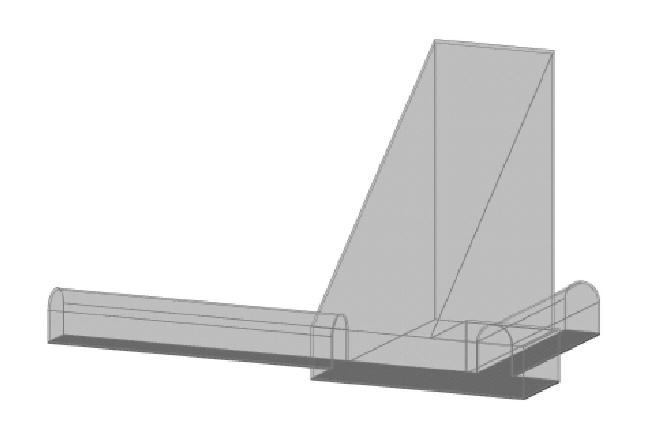
\includegraphics[height=60mm, width=100mm]{view-corner.eps}
        \caption{AutoCAD corner view of plexiglass and aluminum interferometer enclosure. Plexiglass in light gray, aluminum in dark gray. Plexiglass is attached to aluminum with small plexiglass blocks (a refinement to the design), placed three to the long $y$-arm, two to the short $x$-arm, and three to the corner station. The triangular prism is not anchored to the aluminum block. It is open to the bottom so that a projection screen can be inserted, typically atop a flexible rubber sheet. In the World Science Festival exhibit, this projection screen included a photodiode and attached signal cable.}
        \label{plex-view-corner}
        \end{center}
        \end{figure}

        \begin{figure}
        \begin{center}
        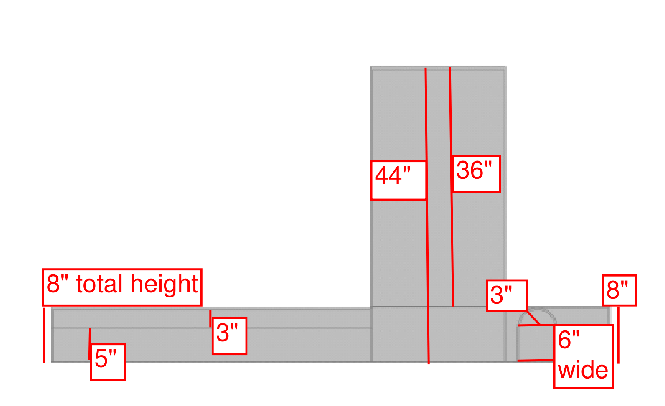
\includegraphics[height=60mm, width=100mm]{view-front.eps}
        \caption{Front view of interferometer aluminum and plexiglass enclosure, with dimensions.}
        \label{plex-view-front}
        \end{center}
        \end{figure}



        \begin{figure}
        \begin{center}
        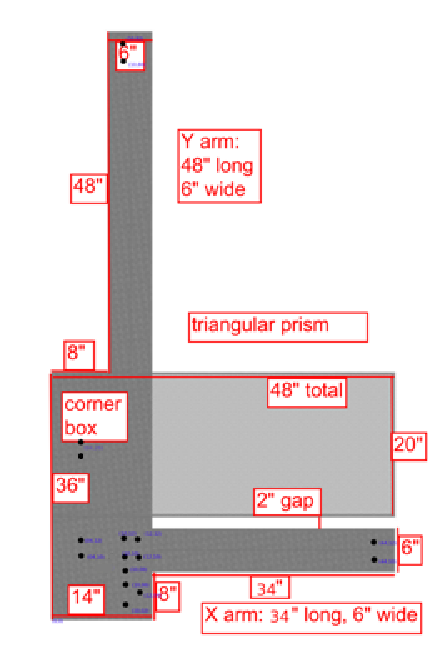
\includegraphics[height=80mm, width=50mm]{view-top-plate-3.eps}
        \caption{Dimensions and hole locations of the aluminum plate (dark gray) relative to plexiglass (light gray), with proposed hole locations given by Table~\ref{aluminum_baseboard_hole_locations}. These hole locations were as tapped.}
        \label{al_top_plate}
        \end{center}
        \end{figure}


	\begin{figure}
	\begin{center}
	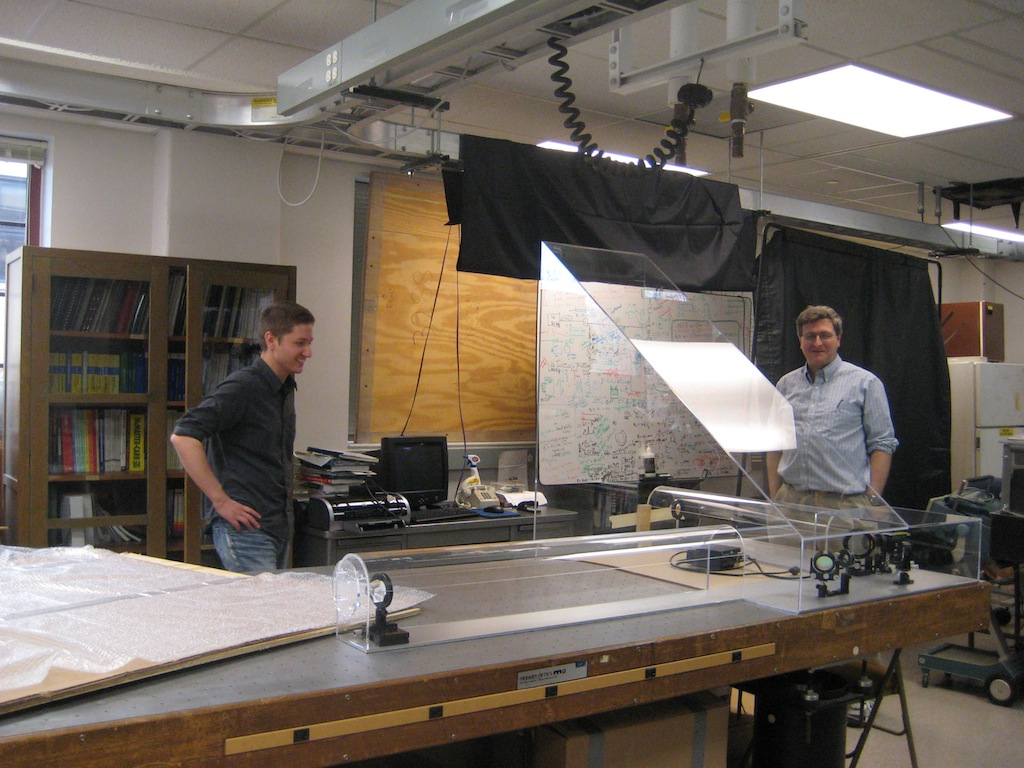
\includegraphics[height=111mm, width=148mm]{WSF_under_construction.eps}
	\caption{Inteferometer assembly in Ann Arbor, Michigan. Projection screen not yet installed. Note the outer end of the $y$-arm (bottom left of photo), with perforated-and-covered plexiglass to allow sound passage. Humans (e.g., Evan Goetz at left, Keith Riles at right) can be protected during alignment processes by laser safety curtains, seen in back.}
	\label{WSF_in_AA}
	\end{center}
	\end{figure}

Should calculate lower bound on $h(t)$ sensitivity based on Saulson, compare to Robert Forward's interferometer.


    \section{Exhibitions: New York City, Portsmouth, Fort Wayne}
    \label{exhibitions}

        World Science Festival interferometer installed.

	\begin{figure}
	\begin{center}
	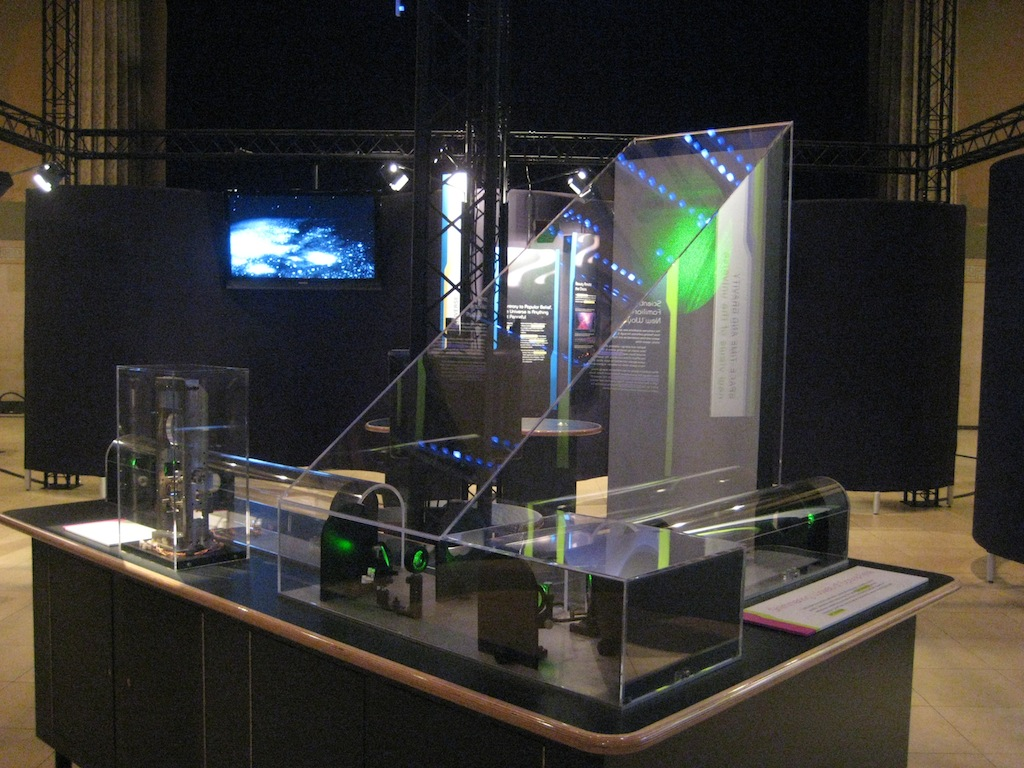
\includegraphics[height=111mm, width=148mm]{WSF_in_NY.eps}
	\caption{World Science Festival interferometer installed in the New York City exhibition hall, June 2010. Optics aligned and baffles installed to protect visitors from scattered light. Also visible: left center, an initial LIGO input mirror and suspension.}
	\label{WSF_IFO_photo}
	\end{center}
	\end{figure}


        \subsection{Exhibit overview}
        \label{exhibit_overview}

            NYC exhibit overview: design, walls, kiosks, displays, interactivities.

        \subsection{World Science Festival 2010}
        \label{WSF2010}

            Success in WSF 2010.

	\begin{figure}
	\begin{center}
	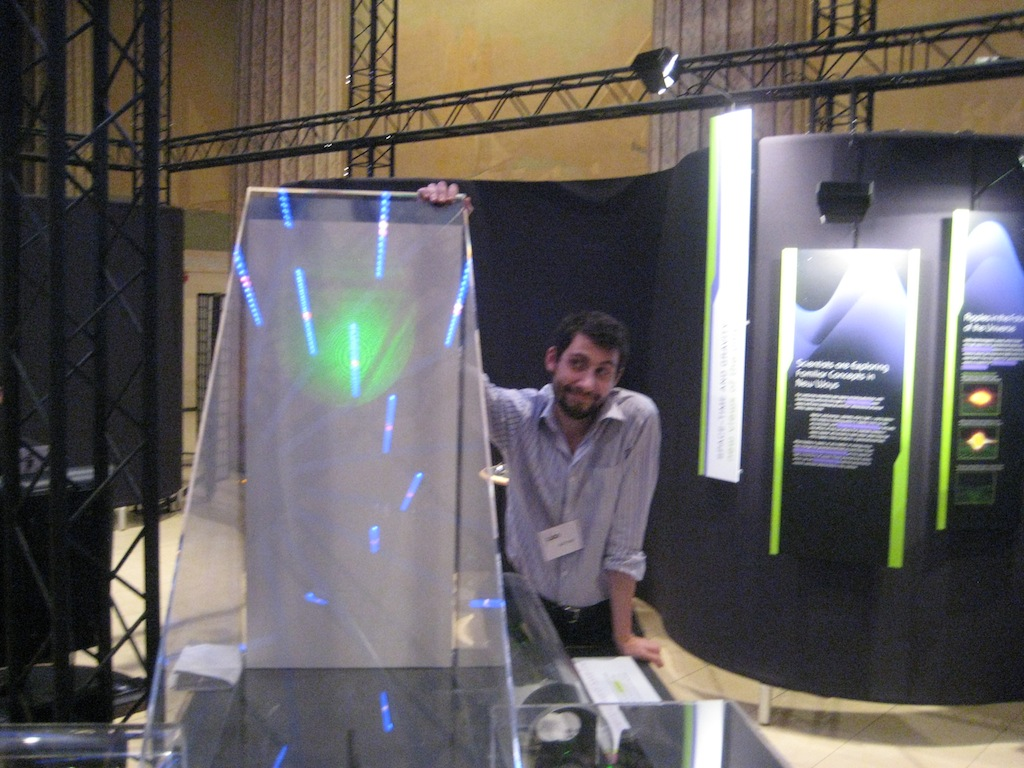
\includegraphics[height=111mm, width=148mm]{WSF_me_NY.eps}
	\caption{Helping to host the exhibit at the World Science Festival. Optics aligned, with fringe pattern, but an edge of the beam-splitter reflection is visible in the projected image. Additional features: the reflected blue lights of the sculpture above and posters of the exhibit.}
	\label{WSF_IFO_me}
	\end{center}
	\end{figure}


        \subsection{Portsmouth and Fort Wayne}
        \label{secondary_installations}

            Secondary installations and future outreach potential.

    \section{Future LIGO outreach}
    \label{future_outreach}

        Epilogue: as of June 2014, the exhibit is safely on display in the Livingston Science and Education center.

        Future LIGO outreach? How to explain a new astronomy.


        --------------------------------------

	%The following is an example of using the commands \textit{ref}
	%and \textit{label}. With these commands theorems, chapters,
	%sections and figurres can be labeld with names in the tex file
	%and then refered to by these names in later tex files. In
	%chapter~\ref{intro} we saw section~\ref{sample_section} or
	%theorem~\ref{sample_theorem}.

	%Lastly, here is how to include a figure. First generate an
	%encapsulated postscript file in xfig, adobe illustrator or
	%some other program. The specific commands are found in
	%\textit{chap2.tex}.

        %\begin{figure}[htb]
        %\centerline{ \epsfig{figure=sample.eps, 
        %height =  1.5 in}}
        %\caption{Sample Figure}
        %\label{sample_figure}
        %\end{figure}

